% !TEX encoding = UTF-8
% !TEX TS-program = pdflatex
% !TEX root = ../Tesi.tex
% !TEX spellcheck = it-IT

%************************************************
\chapter{Modello del dominio}
\label{cap:modello-del-dominio}
%************************************************

\section{Diagramma delle classi}
Si presenta ora il modello delle classi di dominio.
Il modello delle classi di dominio è un modello statico dello spazio del problema che fornisce una visione strutturale ``logica'' del sistema da realizzare.
Il modello delle classi di dominio descrive entità e concetti propri dell'area funzionale che il sistema dovrà implementare.


	%
	% Figura: diagramma delle classi di dominio
	%
	\begin{figure}[h]
		\centering
		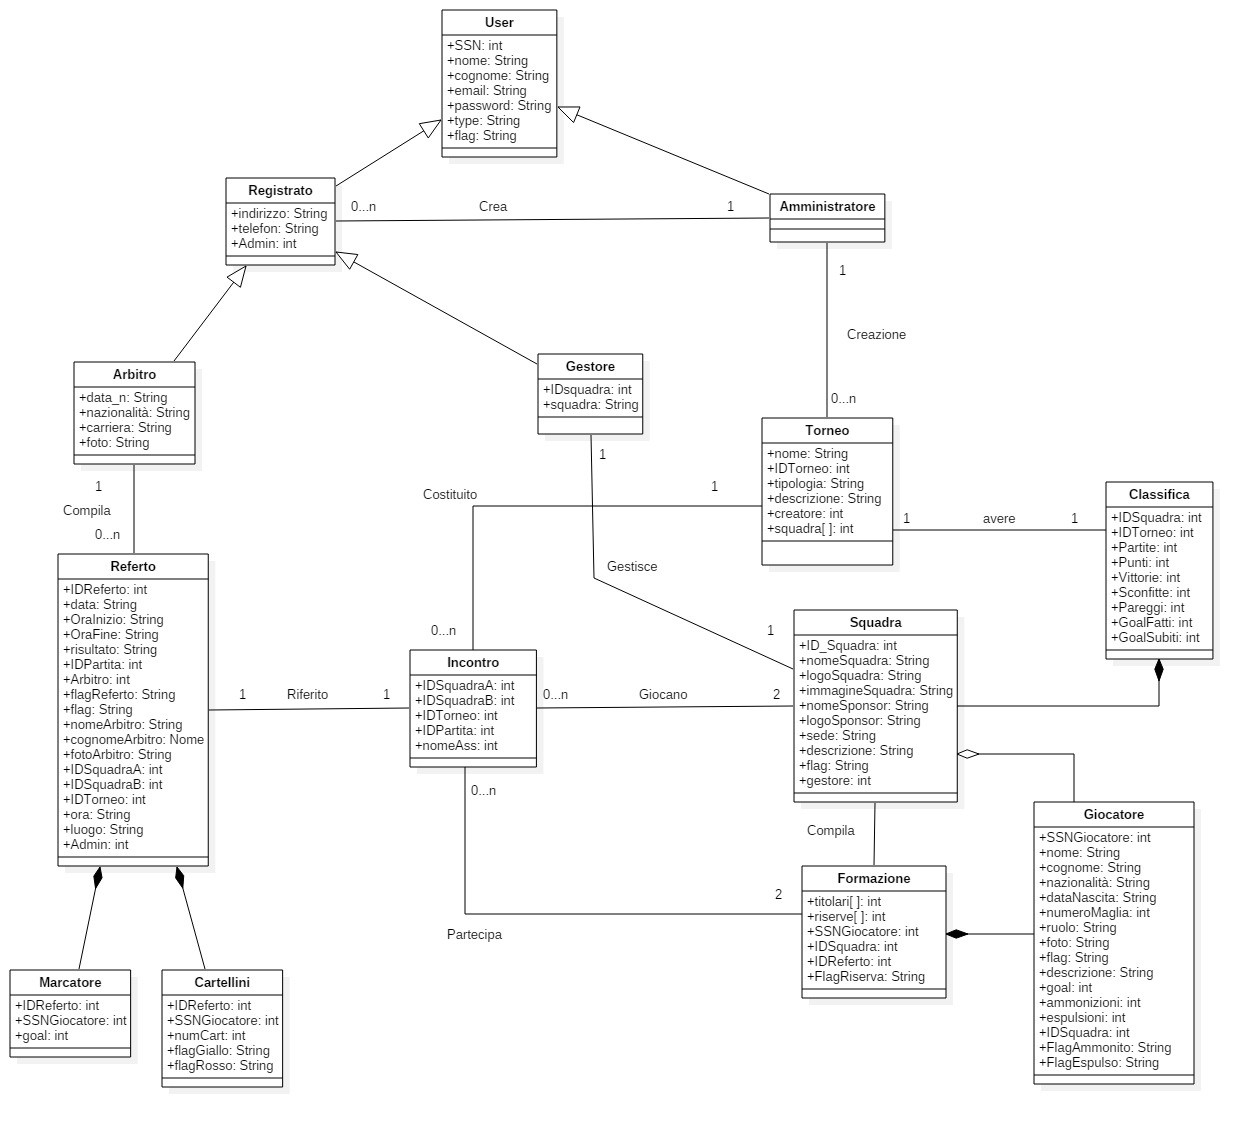
\includegraphics[width=1\textwidth]
		{immagini/cd-sistema}
		
		\caption{Diagramma delle classi di dominio}
	\end{figure}

  \subsection*{N.B.}
  Al fine della leggibilità del diagramma delle classi si è scelto di non inserire i metodi delle varie classi. I metodi delle classi sono specificati nel modello di design delle classi \emph{Entity} a \vref{cap:modello-casi-d'uso}.